\documentclass[11pt]{article}

\usepackage{amsthm, amsmath, amsfonts, mathrsfs}
\usepackage{graphicx}
\usepackage{hyperref}
\hypersetup{
    colorlinks=true,
    linkcolor=blue,
    filecolor=magenta,      
    urlcolor=cyan
    }
\usepackage{tikz}
\usetikzlibrary{topaths,calc,hobby}

\usepackage[margin=0.97in,top=3cm,bottom=2cm, textheight=22.51cm,textwidth=16.51cm, heightrounded,columnsep=0.81cm]{geometry}

\newtheorem{theorem}{Theorem}
\newtheorem{corollary}[theorem]{Corollary}
\newtheorem{property}[theorem]{Property}
\newtheorem{proposition}[theorem]{Proposition}
\newtheorem{lemma}[theorem]{Lemma}
\newtheorem{conjecture}[theorem]{Conjecture}
\newtheorem{problem}[theorem]{Problem}
\newtheorem{definition}[theorem]{Definition}
\newtheorem{example}[theorem]{Example}
\newtheorem{remark}[theorem]{Remark}
\newtheorem{contribution}{Contribution}

\title{Learning in Dynamic Matching Models}
\author{Shu Li \\
        Supervisor:  Ana Bu\v{s}i\'{c}, Jean-Michel Fourneau\\
        INRIA and ENS, PSL University}
\date{}

\newcommand{\fcfm}{\textsc{FCFM}}
\newcommand{\ncond}{\textsc{NCOND}}

\begin{document}

\maketitle
%\tableofcontents
\section{Introduction}\label{sec:intro}

A Matching model is  a triple $( G, \Phi, \mu) $ defined by 
\begin{enumerate}
	\item a matching graph $G=({V},\mathcal{E})$, which is an undirected graph whose nodes in ${V}$ are classes of items 
	and whose edges in $\mathcal{E}$ model the allowed matching of items. $G$ is called the compatibility graph or the Matching graph. Upon arrival, an item is queued if there are no 
	compatible items present in the system.
	
	\item $\Phi$ is a matching policy. It states the couple of items which is chosen
	upon arrival when an arriving item 
	matches one or more items already waiting. Typical matching disciplines are First Come First Matched (FCFM, an analog of First Come First Served in this approach) or Match the Longest Queue. 
	Once they are matched, both items leave the system immediately (no need for service). 
	\item A description of the stochastic processes to 
	model the arrivals. It can be 
	a collection of independent Poisson processes for
	a continuous-time model or a
	distribution of probability over the types of items in discrete time.  In this paper, we assume a continuous time model. 
	The arrival of type $i$ items follow a Poisson process
	with rate $\lambda_i$.  
\end{enumerate} 

We study the FCFM  discipline: upon arrival, if a compatible item is available in the buffer, the arriving item is matched with the oldest such item and the matched pair departs immediately; otherwise, the item is stored in the buffer. Throughout we normalize arrival rates so that $\mu(V)=\sum_{i\in V}\mu_i=1$ . Two structural results underpin our analysis: a necessary stability condition (\ncond) expressed via independent sets~\cite{MaMo18}, and a product-form stationary distribution for the buffer-content chain under {\fcfm}  on connected, non-bipartite graphs~\cite{MBMa21}. Formal notation and these facts are recalled in Section~\ref{sec:prelim}.

We formalize the comparison of interest as follows. For a fixed arrival vector $\mu=(\mu_i)_{i\in V}$ with $\mu(V)=1$, let $G'$ be obtained from $G$ by adding an edge (or adding a self-loop in the multigraph setting). We say a paradox occurs if the stationary total number of items in the buffer on $G'$ exceeds that on $G$, i.e.,
\[
\mathbb{E}[G',\mu]\;>\;\mathbb{E}[G,\mu],
\]
with $\mathbb{E}[G,\mu]:=\sum_{i\in V}\mathbb{E}[Q_i]$ defined under stationarity. Several works report such counterexamples under greedy matching on specific graphs and parameter ranges \cite{CDFB21,BCDF24}. In applications, classes may incur heterogeneous holding costs; we therefore also consider the cost-weighted evaluation $\mathbb{E}[G,\mu,c]:=\sum_{i\in V}c_i\,\mathbb{E}[Q_i]$, used later when we specialize to $K_n$ and $K_n-\{1,2\}$ in Section~\ref{sec:cost}.

On structure, \cite{MaMo18} establishes \textsc{NCOND} and shows that bipartite graphs cannot be positive recurrent under FCFM; \cite{MBMa21} derives the product form on connected, non-bipartite graphs and provides a normalization-by-independent-sets expansion; \cite{BMMR20} extends the construction to multigraphs with self-loops. On paradox evidence under greedy policies, \cite{CDFB21,BCDF24} document instances where adding an edge increases stationary expectation of the total number of items in the buffer on a graph family. 

Under \textsc{FCFM} we make seven contributions. \textbf{(C1)} On \emph{simple} graphs without loops we give purely numerical evidence of paradoxes on very sparse, connected, non-bipartite, star-free instances by evaluating \(\mathbb{E}[G,\mu]\) exactly from the independent–set expansion and comparing \(G\) with \(G+e\). \textbf{(C2)} For \emph{multigraphs} with self-loops we prove an explicit expected-value representation by summing product-form weights over terminal independent sets, extending the simple-graph formula. \textbf{(C3)} Using the formula in (C2) we report numerical paradoxes on graphs with loops and highlight the associated parameter regions; we also pose the open case in which every vertex has a self-loop. \textbf{(C4)} With abandonment, we establish ergodicity on \(K_n\) and derive an exact series expression for the stationary distribution \(\pi_{\emptyset}^{(\delta)}\), yielding \(\mathbb{E}[K_n,\mu,\delta]\) via rapidly convergent series. \textbf{(C5)} For \(K_n-\{1,2\}\) under abandonment, we prove that the CTMC satisfies Ball–Yao strong lumpability and is jumpable; merging \(1\) and \(2\) reduces the model to \(K_{n-1}\), enabling exact evaluation through the \(K_{n-1}\) series. \textbf{(C6)} We design a finite-sum algorithm with certified bounds to compute \(\pi_{\emptyset}^{(\delta)}\) and \(\mathbb{E}[Q_i]\) for \(K_n\) (and, via (C5), for \(K_n-\{1,2\}\)). \textbf{(C7)} Under holding costs \(c=(c_i)\), we obtain closed forms for \(\mathbb{E}[K_n,\mu,c]\) and \(\mathbb{E}[K_n-\{1,2\},\mu,c]\), including a refined empty-state normalizer on \(K_n-\{1,2\}\) that isolates the two-step contribution of the independent set \(\{1,2\}\), and we give cost-weighted paradox examples. 

Section~\ref{sec:prelim} fixes notation, recalls \textsc{NCOND}, and states the product forms and normalising constants for simple graphs and multigraphs. Section~\ref{sec:def-paradox} defines the paradox comparison, reviews illustrative examples, and records a working conjecture. Section~\ref{sec:without-loops} reports (C1). Section~\ref{sec:with-loops} establishes (C2) and presents (C3). Section~\ref{sec:abandonment} develops (C4)–(C6): the continuous-time analysis on \(K_n\), the strong-lumping reduction for \(K_n-\{1,2\}\), and the truncated-series evaluation. Section~\ref{sec:cost} gives the closed forms for \(\mathbb{E}[G,\mu,c]\) on \(K_n\) and \(K_n-\{1,2\}\) and reports cost-weighted(C7). 

\section{Preliminaries}\label{sec:prelim}

We begin with a simple compatibility graph $G=(V,\mathcal{E})$ with $|V|=n$ .
Items of class $i\in V$ arrive according to independent Poisson processes with rates $\mu_i$; throughout we normalize the arrival rate to $\mu(V):=\sum_{i\in V}\mu_i=1$.
Matching is performed under the FCFM: upon arrival, if a compatible item is available in the buffer, the arriving item is matched with the \emph{oldest} such item and the matched pair departs immediately; otherwise, the item is stored in the buffer.

For notational convenience, we write single-vertex arguments with subscripts and set-valued arguments with parentheses; e.g., for $i\in V$ and $S\subseteq V$,
\[
\mu_i:=\mu(\{i\}),\qquad 
\mu(S):=\sum_{i\in S}\mu_i,\qquad
\Gamma_i:=\{\,j\in V:\{i,j\}\in \mathcal{E}\,\},\qquad
\Gamma(S):=\bigcup_{i\in S}\Gamma_i.
\]
When unambiguous we identify a singleton with its element and use shorthands such as $\mu(\Gamma_i)$ for $\mu(\Gamma(\{i\}))$.
Let $W$ denote the (countable) set of admissible words (defined below), including the empty word $\emptyset$.  Let $\mathcal{I}$ denote the family of nonempty independent sets of $G$, i.e., 
$\mathcal{I}:=\{\,I\subseteq V:\ I\neq\emptyset,\ \text{and } \{i,j\}\notin E \text{ for all distinct } i,j\in I\,\}.$


Two simple graphs will be analysed in closed form: the complete graph $K_n$ and the edge-deleted graph $K_n-\{1,2\}$. 
For both, $V_1=\emptyset$, so \eqref{eq:product-form}–\eqref{eq:pi0-general} apply. 
In $K_n-\{1,2\}$ we will use $\Gamma_1=\Gamma_2=\{3,\dots,n\}$, hence $\mu(\Gamma_1)=\mu(\Gamma_2)=\mu(\Gamma(\{1,2\}))$.

Buffer content is represented by a \emph{word} $w=(w(1),\ldots,w(\ell(w)))$ over $V$ listed in order of arrival; write $|w|_i$ for the number of occurrences of $i$ in $w$.
A word $w$ is \emph{admissible} if no two letters in $w$ are adjacent in $G$; equivalently, the set of distinct letters in $w$ is an independent set of $G$.

The buffer-content process $\{W(t)\}_{t\ge0}$ is a continuous-time Markov chain (CTMC) on $W$.
For $w\in W$ and $i\in V$, define the update operator $A_i(w)$ as follows:
\begin{itemize}\itemsep0.2em
	\item If $w$ contains a letter in $\Gamma_i$, let $t=\min\{k:\ w(k)\in\Gamma_i\}$ (the \emph{oldest} compatible letter). Then $A_i(w)$ is obtained by deleting $w(t)$ from $w$ (the arrival matches and both depart).
	\item Otherwise, $A_i(w)$ appends $i$ to the end of $w$ (the arrival is stored).
\end{itemize}
The generator acts on bounded functions $f:W\to\mathbb{R}$ as
\[
\mathcal{L}f(w)\;=\;\sum_{i\in V}\mu_i\bigl[f\bigl(A_i(w)\bigr)-f(w)\bigr].
\]
All stationary statements below presuppose positive recurrence of this CTMC (e.g., when NCOND holds; see Theorem~\ref{thm:ncond}).

The stability region of $(G, \Phi)$ is the set of probability measures $\mu$ on $\mathcal{V}$ such that the natural Markov chain of $(G,\Phi,\mu)$ is positive recurrent.

\begin{theorem}[Stability condition (\textsc{NCOND}), {\cite[Thm.~2]{MaMo18}}]\label{thm:ncond}
	For every independent set $I\in\mathcal{I}$,
	\begin{equation}\label{eq:ncond}
		\mu(I)\;<\;\mu\!\bigl(\Gamma(I)\bigr).
	\end{equation}
	In particular, if $G$ is bipartite with bipartition $(A,B)$, applying \eqref{eq:ncond} to $I=A$ and $I=B$ yields a contradiction; hence such graphs cannot be positive recurrent under \fcfm.
\end{theorem}

On connected, non-bipartite simple graphs, and whenever the chain is positive recurrent, the stationary distribution admits the following product form.
\begin{theorem}[Product form {\cite{MBMa21}}]\label{thm:pf-simple}
	Let $G$ be a connected, non-bipartite simple graph. For any admissible word $w=(w(1),\ldots,w(\ell(w)))\in W$,
	\begin{equation}\label{eq:product-form}
		\pi(w)\;=\;\pi_{\emptyset}\;\prod_{k=1}^{\ell(w)}\frac{\mu_{\,w(k)}}{\mu\!\bigl(\Gamma(\{w(1),\ldots,w(k)\})\bigr)}\,,
	\end{equation}
	where the normalizing constant is
	\begin{equation}\label{eq:pi0-general}
\pi_{\emptyset}^{-1}=1+\sum_{I\in\mathcal{I}}\sum_{\sigma\in \mathfrak{S}_{|I|}}\prod_{k=1}^{|I|}
\frac{\mu_{i_{\sigma(k)}}}{\mu\bigl(\Gamma(\{i_{\sigma(1)},\ldots,i_{\sigma(k)}\})\bigr)-\mu\bigl(\{i_{\sigma(1)},\ldots,i_{\sigma(k)}\}\bigr)},
	\end{equation}
	with $I=\{i_1,\ldots,i_{|I|}\}$ and $\mathfrak{S}_{|I|}$ the permutation group on $|I|$ elements.
\end{theorem}

Assuming positive recurrence, let $W_\infty$ be a random word with law $\pi(\cdot)$ on $W$, i.e., $\mathbb{P}\{W_\infty=w\}=\pi(w)$ for all $w\in W$.
For $i\in V$,
\begin{equation}\label{eq:defQi}
	Q_i:=|W_\infty|_i,\qquad 
	\mathbb{E}[Q_i]=\sum_{w\in W}\pi(w)\,|w|_i.
\end{equation}

\noindent
Summing the product-form weights in Theorem~\ref{thm:pf-simple} by grouping admissible words according to their terminal independent set yields an explicit evaluation of the total stationary number of items in the buffer.

\begin{theorem}[Expectation, \cite{CDFB21}]\label{thm:EV-simple}
For all independent sets $\mathcal{I} \in \mathbb{I}$, consider an ordered version of $\mathcal{I}$ noted $\mathcal{I}^o=$ $\left\{i_1, \cdots, i_{|\mathcal{I}|}\right\}$, we note $\sigma$ a permutation of its elements, i.e $\mathcal{I}^{\sigma(o)}=\left\{i_{\sigma(1)}, \cdots, i_{\sigma(|\mathcal{I}|)}\right\}$ and $\mathfrak{S}_{|\mathcal{I}|}$ the set of all permutations on the nodes of $\mathcal{I}$. We define:
\[
T_{\mathcal{I}^o}=\prod_{k=1}^{|\mathcal{I}|} 
\frac{\mu_{i_k}}
{ \mu(\Gamma (\left\{i_1, \cdots, i_k\right\}))
	-\mu(\left\{i_1, \cdots, i_k\right\})}.
\]
Furthermore $T_{\mathcal{I}}=\sum_{\sigma \in \mathfrak{S}_{|\mathcal{I}|}} T_{\mathcal{I}^{\sigma(o)}}$.
We also define: 
\[
E_{\mathcal{I}^o}=\sum_{l=1}^{|\mathcal{I}|} 
\frac{\mu(\Gamma(\{i_1, \cdots, i_l\})}{ \mu(\Gamma( \{ i_1, \cdots, i_l \})) -\mu(\{i_1, \cdots, i_l\})} \prod_{k=1}^{|\mathcal{I}|} \frac{\mu_{i_k}}
{ \mu(\Gamma( \{ i_1, \cdots, i_k \})) -\mu(\{i_1, \cdots, i_k\})}
\]
Finally,  $E_{\mathcal{I}}=\sum_{\sigma \in \mathfrak{G}_{|\mathcal{I}|}} E_{\mathcal{I}^{\sigma(o)}}$. 
$\mathbb{E}[G, \mu ]$  can be rewritten as a finite sum over all independent sets, i.e 
\begin{equation}\label{eq:EV-simple}
	\mathbb{E}[G,\mu]=\left(1+\sum_{\mathcal{I} \in \mathbb{I}}T_{\mathcal{I}}\right)^{-1}\left(\sum_{\mathcal{I}\in \mathbb{I}} E_{\mathcal{I}}\right)
\end{equation}  
\end{theorem}

When self loops are allowed. Thus the compatibility graph becomes a multigraph. Let $G=(\mathcal{V}, \mathcal{E})$ be a multigraph with the nodes partition $\mathcal{V}=\mathcal{V}_1\cup\mathcal{V}_2$ where $\mathcal{V}_1=\{i\in \mathcal{V}\mid \{i,i\}\in \mathcal{E}\}$ and $\mathcal{V}_2 = \mathcal{V}\setminus \mathcal{V}_1$. Denote by $\mathbb{I} (\check{G})$ the family of independent sets of 
$\check{G}=(\mathcal{V},\mathcal{E}\setminus\{(i,i)\mid i\in\mathcal{V}_1\})$.

\begin{theorem}[Product form {\cite[Theorem 4.5]{BMMR20}}]\label{th:prod-multi}
	Assume FCFM policy and ergodicity.  
	For any word $w=(w_1,\dots,w_q)\in W$,
	\begin{equation}
		\pi(w)= \pi({\emptyset}) \bar{\pi}(w)  =  \pi({\emptyset}) \prod_{l=1}^{q}\frac{\mu(\{w_l\})}{\mu\bigl(\Gamma(\{w_1,\dots,w_l\})\bigr)},
	\end{equation}
	where
	\[
	\pi({\emptyset})^{-1}=1+\sum_{\mathcal{I}\in\mathbb{I}(\check{G})}\sum_{\sigma\in \mathfrak{S}_{|\mathcal{I}|}}
	\prod_{k=1}^{|\mathcal{I}|}
	\frac{\mu(\{e_{\sigma(k)}\})}{
		\mu\bigl(\Gamma(\{e_{\sigma(1)},\dots,e_{\sigma(k)}\})\bigr)-\mu\bigl(\{e_{\sigma(1)},\dots,e_{\sigma(k)}\}\cap \mathcal{V}_2\bigr)}. \]
\end{theorem} 

\section{Performance paradoxes in matching systems}\label{sec:def-paradox}

Building on the preliminaries, we evaluate stationary performance on a compatibility graph $G=(V,E)$ under \textsc{FCFM} via the total number of items in the buffer
\[
\mathbb{E}[G,\mu]\;=\;\sum_{i\in V}\mathbb{E}[Q_i],
\]
defined under positive recurrence. For loop-free graphs, $\mathbb{E}[G,\mu]$ admits the explicit independent-set expansion in \eqref{eq:EV-simple}; for graphs with self-loops, we use the multigraph product form and normalization in \eqref{eq:exp-multi}. A common design operation is to \emph{add compatibility}—formally, to pass from $G$ to a supergraph $G'$ on the same vertex set by adding an edge (or, in the multigraph setting, a self-loop). Intuition might suggest that such an operation should not worsen stationary performance; the paradoxes studied here show that this monotonicity need not hold.

\begin{definition} [Performance Paradox] 
	For some arrival rates $\mu$, we have a performance paradox, if  $\mathbb{E} [G+e, \mu]  > \mathbb{E} [G, \mu] $. 
\end{definition}

\begin{property} [First Performance Paradox \cite{CDFB21}]  
	Let $K_4$ be the complete graph with $4$ nodes.
	For some arrival rates $\mu$, we have proved that  $$\mathbb{E} [K_4-(1,2), \mu]  < \mathbb{E} [K_4, \mu] .$$ 
\end{property}


The analysis in \cite{CDFB21} requires one combinatorial notion. The {bottleneck set}, denoted $BS(G,\lambda)$ throughout this paper, is defined as
\[
BS (G,\mu) =\{I \in \mathcal{I}\mid argmin(\mu(\Gamma(I))-\mu(I))\}.
\]

As it is difficult to use the formula on the expectation, we have developed in \cite{BCDF24} some "lifting theorems" to
explain how one can build large compatibility graphs and arrival rates based on small compatibility graphs. We have 
proved that the existence of performance paradoxes on small graphs implies the existence of such paradoxes 
on large graphs. Then from the initial seed graph (i.e. $K_4-(1,2)$ in \cite{CDFB21}) 
we have obtained an infinite set of graphs with paradoxes with the help of the JOIN operation defined as follows. 
\begin{definition} [JOIN $\bowtie$]. Let $G1=(V1,E1) $ and  $G2=(V2,E2) $ two arbitrary graphs, 
	the join of $G1$ and $G2$ (denoted as $G1 \bowtie G2$) is defined by the set of nodes $V1 \cup V2$ and the set 
	of edges $E1 \cup E2 \cup V1 \times V2$, where $\times $ is the Cartesian product.  
\end{definition} 
\begin{property} [Construction of Performance Paradox \cite{BCDF24}] 
	\label{family}
	Performance paradoxes exist for graphs $IN_n \bowtie (K_4 -(1,2)) $ where $ IN_n$ is the graph with $n$ isolated nodes.   
\end{property}

Motivated by the definition and examples above, we have a conjecture.
\begin{conjecture}
A star is not needed and the compatibility graph may have a degree equal to 1
\end{conjecture}

In Section~\ref{sec:without-loops} we begin this test on simple graphs, focusing on sparse instances without star subgraphs and allowing degree-$1$ vertices, in order to probe the necessity claims embodied in the conjecture.

\section{Graphs without loops}\label{sec:without-loops}

We now turn to star-free compatibility graphs. The goal is to empirically probe the conjecture stated at the end of Section~\ref{sec:def-paradox}: namely, that star substructures are not necessary for paradoxes and that paradoxes may occur even when the graph admits degree-$1$ vertices. All evaluations use the explicit formula from Section~\ref{sec:prelim} under \textsc{NCOND} for both $G$ and $G+e$.


\begin{contribution}
We provide \emph{numerical} evidence of paradoxes on simple star-free graphs. 
For each candidate graph $G$ we sample $\mu$ under NCOND, evaluate $\mathbb{E}[G,\mu]$ via \eqref{eq:EV-simple}, and compare it to $\mathbb{E}[G+e,\mu]$ after adding a single edge $e$. 
All the  instances are reported below; full scripts and algorithms are in \cite{li2025b}.
\end{contribution}

A simple graph $G$ is \emph{star-free} if it contains no induced subgraph isomorphic to a star.
Because bipartite graphs cannot be positive recurrent under \fcfm\ (Theorem~\ref{thm:ncond}), we focus on connected, non-bipartite, star-free, non-complete graphs.
Both “connected” and “star-free” are monotone under edge addition, so if they hold for $G$ they also hold for $G+e$.
An enumeration shows that the smallest star-free, non-bipartite examples have five vertices and contain a single odd cycle. 
We therefore begin with $C_5$ and $F_1$ (Fig.~\ref{fig:twoc5}), then enlarge to six vertices with $F_3$ (two distinct odd cycles), and finally examine the $7$-cycle $C_7$.
In all cases we evaluate $\mathbb{E}[G,\mu]$ using \eqref{eq:EV-simple} with $\mu(V)=1$.

\subsection{Graphs $C_5$ and $F_1$}

\begin{figure}[htbp]
	\centering
	\begin{minipage}{0.23\textwidth}
		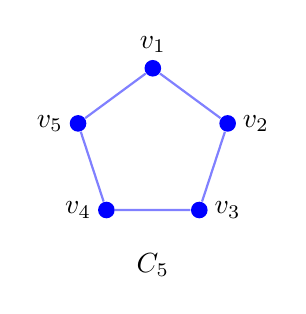
\begin{tikzpicture}[scale=1, vertex/.style={minimum width=6pt, circle,fill=blue, inner sep=0pt}]
			\foreach \i/\x/\y in {1/0/1, 2/0.95/0.3, 3/0.59/-0.8, 4/-0.59/-0.8, 5/-0.95/0.3} {
				\node[vertex] (v\i) at (\x,\y) {};
			}
			\node[above=2pt] at (v1){$v_1$};
			\node[right=2pt] at (v2){$v_2$};
			\node[right=2pt] at (v3){$v_3$};
			\node[left=2pt] at (v4){$v_4$};
			\node[left=2pt] at (v5){$v_5$};
			\draw[blue!50,thick] (v1) -- (v2) -- (v3) -- (v4) -- (v5) -- (v1);
			\node(c5) at (0,-1.5){$C_5$};
		\end{tikzpicture}
	\end{minipage}\hspace{3pt}
	\begin{minipage}{0.23\textwidth}
		\centering
		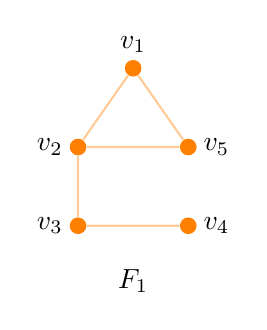
\begin{tikzpicture}[scale=1, vertex/.style={minimum width=6pt, circle, fill=orange, inner sep=0pt}]
			\node[vertex] (z1) at (0,1){};
			\node[above=2pt] at (z1) {$v_1$};
			\node[vertex] (z2) at (-0.7,0){};
			\node[left=2pt] at (z2) {$v_2$};
			\node[vertex] (z3) at (-0.7,-1){};
			\node[left=2pt] at (z3) {$v_3$};
			\node[vertex] (z4) at (0.7,-1){};
			\node[right=2pt] at (z4) {$v_4$};
			\node[vertex] (z5) at (0.7,0){};
			\node[right=2pt] at (z5) {$v_5$};
			\draw[orange!40,thick](z2)--(z5)--(z1)--(z2)--(z3)--(z4);
			\node at (0,-1.7){$F_1$};
		\end{tikzpicture}
	\end{minipage}\hspace{3pt}
	\begin{minipage}{0.23\textwidth}
		\centering
		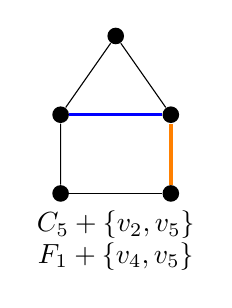
\begin{tikzpicture}[scale=1, vertex/.style={minimum width=6pt, circle, fill=black, inner sep=0pt}]
			\node[vertex] (z1) at (0,1){};
			\node[vertex] (z2) at (-0.7,0){};
			\node[vertex] (z3) at (-0.7,-1){};
			\node[vertex] (z4) at (0.7,-1){};
			\node[vertex] (z5) at (0.7,0){};
			\draw (z5)--(z1)--(z2)--(z3);
			\draw[blue, very thick](z2)--(z5);
			\draw (z3)--(z4);
			\draw[orange,very thick](z4)--(z5);
			\node at (0,-1.4){$C_5+\{v_2,v_5\}$};
			\node at (0,-1.8){$F_1+\{v_4,v_5\}$};
		\end{tikzpicture}
	\end{minipage}
	\caption{Star-free graphs on five vertices: $C_5$ and $F_1$.}
	\label{fig:twoc5}
\end{figure}

The cycle $C_5$ has five vertices, five edges, is connected, and has $10$ independent sets.
Using \eqref{eq:EV-simple}, for
\[
\mu=(0.111,\ 0.10575,\ 0.179426,\ 0.35046,\ 0.253364),
\]
replacing $C_5$ by $C_5+\{v_2,v_5\}$ increases the expectation from $7.86$ to $8.17$; a performance paradox.
A similar upward shift occurs when augmenting $F_1$ to $F_1+\{v_4,v_5\}$:
for
\[
\mu=(0.266025,\ 0.11005,\ 0.210855,\ 0.14145,\ 0.27162),
\]
the expected total number of items grows from $16.069$ to $16.89$.
In these instances the bottleneck independent sets (as revealed by the smallest denominator in \eqref{eq:EV-simple}) are $\{v_1,v_4\}$ for the first example and $\{v_3,v_5\}$ for the second.
(All vectors satisfy \eqref{eq:ncond} and are normalized to $\mu(V)=1$; see \cite{li2025b} for exact computations and seeds.)

\subsection{$F_3$: star-free with two odd cycles}

\begin{figure}[htbp]
	\centering
	\begin{minipage}{0.5\textwidth}
		\centering
		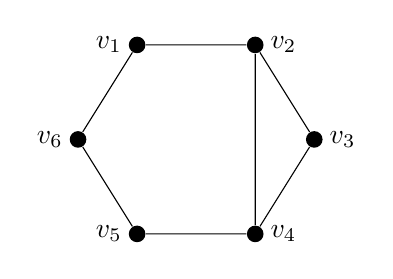
\begin{tikzpicture}[scale=1.5, vertex/.style={minimum width=6pt, circle, fill=black, inner sep=0pt}]
			\node[vertex](v1) at (-0.5,0.8){};
			\node[left=2pt] at (v1){$v_1$};
			\node[vertex](v2) at (0.5,0.8){};
			\node[right=2pt] at (v2){$v_2$};
			\node[vertex](v3) at (1,0){};
			\node[right=2pt] at (v3){$v_3$};
			\node[vertex](v4) at (0.5,-0.8){};
			\node[right=2pt] at (v4){$v_4$};
			\node[vertex](v5) at (-0.5,-0.8){};
			\node[left=2pt] at (v5){$v_5$};
			\node[vertex](v6) at (-1,0){};
			\node[left=2pt] at (v6){$v_6$};
			\draw (v1)--(v2)--(v3)--(v4)--(v5)--(v6)--(v1);
			\draw(v2)--(v4);
		\end{tikzpicture}
	\end{minipage}
	\hspace{3pt}
	\begin{minipage}{0.4\textwidth}
		\centering
		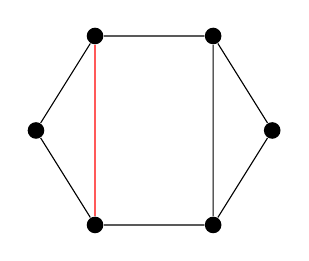
\begin{tikzpicture}[scale=1.5, vertex/.style={minimum width=6pt, circle, fill=black, inner sep=0pt}]
			\node[vertex](v1) at (-0.5,0.8){};
			\node[vertex](v2) at (0.5,0.8){};
			\node[vertex](v3) at (1,0){};
			\node[vertex](v4) at (0.5,-0.8){};
			\node[vertex](v5) at (-0.5,-0.8){};
			\node[vertex](v6) at (-1,0){};
			\draw (v1)--(v2)--(v3)--(v4)--(v5)--(v6)--(v1);
			\draw(v2)--(v4);
			\draw[red](v1)--(v5);
		\end{tikzpicture}
	\end{minipage}
	\caption{$F_3$ and $F_3+\{v_1,v_5\}$. }
	\label{fig:twocycle}
\end{figure}

Graph $F_3$ is obtained by inserting the edge $\{v_2,v_4\}$ into $C_6$, producing two distinct odd cycles of lengths $3$ and $5$ and $15$ independent sets.
For
\[
\mu=(0.231787,\ 0.462366,\ 0.14472,\ 0.127484,\ 0.00342,\ 0.030223),
\]
we obtain $\mathbb{E}[F_3,\mu]=31.59$ and $\mathbb{E}[F_3+\{v_1,v_5\},\mu]=31.71$; thus adding the edge $\{v_1,v_5\}$ increases the stationary total number of items in the buffer.
In both graphs, the bottleneck independent set is $\{v_2,v_6\}$.
(Computations reproduced from \cite{li2025b}.)

\subsection{$C_7$: paradox on a simple cycle}

\begin{figure}[htbp]
	\centering
	\begin{minipage}{0.4\textwidth}
		\centering
		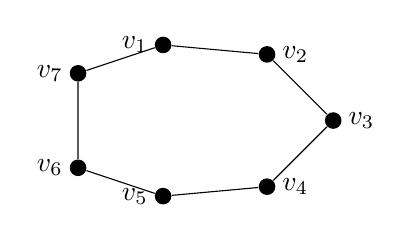
\begin{tikzpicture}[scale=1.2, vertex/.style={minimum width=6pt, circle, fill=black, inner sep=0pt}]
			\node[vertex](v1) at (-0.5,0.8){};
			\node[left=2pt] at (v1){$v_1$};
			\node[vertex](v2) at (0.6,0.7){};
			\node[right=2pt] at (v2){$v_2$};
			\node[vertex](v3) at (1.3,0){};
			\node[right=2pt] at (v3){$v_3$};
			\node[vertex](v4) at (0.6,-0.7){};
			\node[right=2pt] at (v4){$v_4$};
			\node[vertex](v5) at (-0.5,-0.8){};
			\node[left=2pt] at (v5){$v_5$};
			\node[vertex](v6) at (-1.4,-0.5){};
			\node[left=2pt] at (v6){$v_6$};
			\node[vertex](v7) at (-1.4,0.5){};
			\node[left=2pt] at (v7){$v_7$};
			\draw (v1)--(v2)--(v3)--(v4)--(v5)--(v6)--(v7)--(v1);
		\end{tikzpicture}
	\end{minipage}
	\hspace{3pt}
	\begin{minipage}{0.4\textwidth}
		\centering
		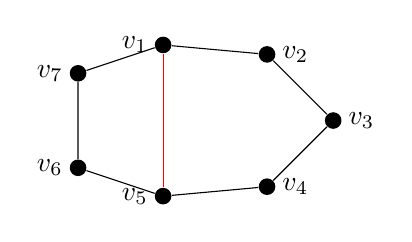
\begin{tikzpicture}[scale=1.2, vertex/.style={minimum width=6pt, circle, fill=black, inner sep=0pt}]
			\node[vertex](v1) at (-0.5,0.8){};
			\node[left=2pt] at (v1){$v_1$};
			\node[vertex](v2) at (0.6,0.7){};
			\node[right=2pt] at (v2){$v_2$};
			\node[vertex](v3) at (1.3,0){};
			\node[right=2pt] at (v3){$v_3$};
			\node[vertex](v4) at (0.6,-0.7){};
			\node[right=2pt] at (v4){$v_4$};
			\node[vertex](v5) at (-0.5,-0.8){};
			\node[left=2pt] at (v5){$v_5$};
			\node[vertex](v6) at (-1.4,-0.5){};
			\node[left=2pt] at (v6){$v_6$};
			\node[vertex](v7) at (-1.4,0.5){};
			\node[left=2pt] at (v7){$v_7$};
			\draw (v1)--(v2)--(v3)--(v4)--(v5)--(v6)--(v7)--(v1);
			\draw[red](v1)--(v5);
		\end{tikzpicture}
	\end{minipage}
	\caption{$C_7$ and $C_7+\{v_1,v_5\}$.}
	\label{fig:cycle7}
\end{figure}

For the simple odd cycle $C_7$ (with $28$ independent sets), take
\[
\mu=(0.045206,\ 0.240384,\ 0.303789,\ 0.146114,\ 0.132526,\ 0.111772,\ 0.020209).
\]
Then $\mathbb{E}[C_7,\mu]=129.56$ and $\mathbb{E}[C_7+\{v_1,v_5\},\mu]=137.87$, again a performance paradox.
Both graphs share the bottleneck independent set $\{v_2,v_4,v_6\}$.
Full logs and verification are provided in \cite{li2025b}.

\section{Graphs with loops}\label{sec:with-loops}

We compare graphs on the same vertex set $(V,\mu)$ under the same policy and say a paradox occurs if the evaluation on $G'$—obtained from $G$ by adding an edge (or a self-loop in the multigraph case)—exceeds that on $G$.
We work throughout under \textsc{FCFM} with arrivals $\mu=(\mu_i)_{i\in V}$ normalized by $\mu(V)=1$, and we use the multigraph notation of Section~\ref{sec:prelim}: self-loop classes $V_1$, loop-free classes $V_2=V\setminus V_1$, loop-deleted graph $\check{G}=(V,\mathcal{E})$, neighborhoods $\Gamma_i$ and $\Gamma(S)$ defined on $\check{G}$, and admissible words $W$. The necessary stability condition (\textsc{NCOND}) and the product-form stationary distribution with normalizing constant $\pi_{\emptyset}$ are recalled in Theorem~\ref{th:prod-multi}.

We now rewrite the sum over all words $w$ as a finite sum over independent sets of $\check{G}$. 
For $\mathcal{I}\in\mathbb{I}(\check G)$,  fix an arbitrary ordering 
$\mathcal{I}^o=\{e_1,\dots,e_{|\mathcal{I}|}\}$. Given a permutation $\sigma$ 
of the index set $\{1,\dots,|\mathcal{I}|\}$, define the reordered 
list $\mathcal{I}^{\sigma(o)}=\{e_{\sigma(1)},\dots,e_{\sigma(|\mathcal{I}|)}\},$
that is, the sequence obtained by applying 
$\sigma$ to the ordered version $\mathcal{I}^o$. 
We denote $\mathcal{I}_k^o$ as the first $k$ elements of $\mathcal{I}^o$.
Let $\mathcal{J}_k^o=\mathcal{I}_k^o\cap \mathcal{V}_2$. 
We define 
\begin{equation}
	T_{\mathcal{I}^o}=\prod_{k=1}^{|\mathcal{I}|}\frac{\mu(\{e_{k}\})}{\mu\Bigl(\Gamma\bigl(\mathcal{I}_k^o\bigr)\Bigr)-\mu\Bigl(\mathcal{J}_k^o\Bigr)},
\end{equation}
and $T_{\mathcal{I}}=\sum_{\sigma \in \mathfrak{S}_{|\mathcal{I}|}} T_{\mathcal{I}^{\sigma(o)}}$. Thus $\pi(\emptyset) = (1 +T_{\mathcal{I}})^{-1}$. 
We also define
\begin{equation}
	E_{\mathcal{I}^o}=\sum_{l=1}^{|\mathcal{I}|}
	\frac{\mu\Bigl(\Gamma\bigl(\mathcal{I}_l^o\bigr)\Bigr)}
	{\mu\Bigl(\Gamma\bigl(\mathcal{I}_l^o\bigr)\Bigr)-
\mu\Bigl(\mathcal{J}_l^o\Bigr)}\prod_{k=1}^{|\mathcal{I}|}
	\frac{\mu(\{e_{k}\})}{\mu\Bigl(\Gamma\bigl(\mathcal{I}_k^o\bigr)\Bigr)-
\mu\Bigl(\mathcal{J}_k^o\Bigr)},   
\end{equation}
and $E_{\mathcal{I}}=\sum_{\sigma \in \mathfrak{S}_{|\mathcal{I}|}} E_{\mathcal{I}^{\sigma(o)}}$.

\begin{contribution}[Expectation]\label{cor:exp-multi}
The expected number of items in steady state is
\begin{equation}\label{eq:exp-multi}
\mathbb{E}[G,\mu]=\Bigl(1+\sum_{\mathcal{I}\in\mathbb{I}(\check G)}T_\mathcal{I}\Bigr)^{-1}\sum_{\mathcal{I}\in\mathbb{I}(\check G)}E_\mathcal{I}.
\end{equation}
\end{contribution}

\begin{proof}
	By Theorem~\ref{th:prod-multi}, we obtain the normalization $\pi(\emptyset)^{-1}=1+\sum_{\mathcal{I}}T_\mathcal{I}$, which implies $\pi(\emptyset)=(1+\sum_{\mathcal{I}}T_\mathcal{I})^{-1}$.  Now, in view of Equation (2), it suffices to prove that 
	$$\sum_{w}|w|\overline{\pi}(w)=\sum_{\mathcal{I}}X_\mathcal{I}.$$
	We now rewrite the sum over all words $w$ as a finite sum over independent sets of $\check{G}$.  For $\mathcal{I}\in\mathbb{I}(\check{G})$, let 
	$$
	\overline{\pi}_{\mathcal{I}} =\sum_{\substack{w\in W:\\ \mathrm{mubet}(w)=\mathcal{I}}} |w|\overline{\pi}(w),
	$$
	where “$\mathrm{mubet}(w)=\mathcal{I}$” means that the set of distinct nodes (classes) appearing in $w$ is exactly $\mathcal{I}\in\mathbb{I}(\check{G})$ with $|\mathcal{I}|=m$. Let $\mathcal{I}^o=(i_1,\dots,i_{m})$ be an arbitrary ordering (permutation) of $\mathcal{I}$. 
	We denote $\mathcal{I}_k^o$ as the first $k$ elements of $\mathcal{I}^o$. 
	Let $\mathcal{J}=\mathcal{I}\cap \mathcal{V}_2$, $\mathcal{J}_k=\mathcal{I}_k\cap \mathcal{V}_2$ and $\mathcal{J}_k^o=\mathcal{I}_k^o\cap \mathcal{V}_2$. Consider words $w$ whose first occurrences of distinct letters follow the order $i_1,\dots,i_{m}$.  
	Label the lengths between first occurrences as follows: For $l\leq k<m$, and $i_k \in J^o_k$, let $p_{l}^k$ denote the number of times the letter $i_l$ appears between the first occurrences of $i_k$ and $i_{k+1}$ (exclusive).
	For any $i\in\mathcal{I}\cap\mathcal{V}_1$, the letter $i$ appears zero times between $i_k$ and $i_{k+1}$, since nodes in $\mathcal{V}_1$ have self-loops.
	Since there is no $i_{m+1}$, we denote $p_l^m$ is the number of $i_l$ from the first $i_m$ to the end of state.
	Define $$n_k= \sum_{l=1}^{k} p_{l}^k,$$ summing over all $i_l \in \mathcal{J}$.
	Then any such word $w$ has total length 
	$|w|=|\mathcal{I}|+\sum_{k=1}^{|\mathcal{I}|} n_k$. 
	The corresponding multinomial coefficient is
	$$\binom{n_k}{\{p_l^k\}_{\{i_l\in\mathcal{J}_k^o\}}}=\frac{n_k!}{\prod_{i_l\in\mathcal{J}_k^o} {p_l^k}!}.$$
	The contribution from a word $w^*=i_1,\dots,i_2\dots,i_m,\dots$ is $$
	\Bigl[\frac{\mu(i_1)}{\mu(\mathcal{E}(\mathcal{I}^o_1))}
	\Bigl(\frac{\mu(i_1)}{\mu(\mathcal{E}(\mathcal{I}^o_1))}\Bigr)^{p_1^1}\Bigr]
	\Bigl[\frac{\mu(i_2)}{\mu(\mathcal{E}(\mathcal{I}^o_2)}
	\Bigl(\frac{\mu(i_1)}{\mu(\mathcal{E}(\mathcal{I}^o_2)}\Bigr)^{p_1^2}
	\Bigl(\frac{\mu(i_2)}{\mu(\mathcal{E}(\mathcal{I}^o_2)}\Bigr)^{p_2^2}\Bigr]\dots
	\Bigl[\frac{\mu(i_k)}{\mu(\mathcal{E}(\mathcal{I}^o_k)}
	\Bigl(\frac{\mu(i_1)}{\mu(\mathcal{E}(\mathcal{I}^o_k)}\Bigr)^{p_1^k}\dots
	\Bigl(\frac{\mu(i_k)}{\mu(\mathcal{E}(\mathcal{I}^o_k)}\Bigr)^{p_k^k}\Bigr]$$ $$\dots\Bigl[\frac{\mu(i_m)}{\mu(\mathcal{E}(\mathcal{I}^o_m)}
	\Bigl(\frac{\mu(i_1)}{\mu(\mathcal{E}(\mathcal{I}^o_m)}\Bigr)^{p_1^m}\dots
	\Bigl(\frac{\mu(i_m)}{\mu(\mathcal{E}(\mathcal{I}^o_m)}\Bigr)^{p_m^m}\Bigr]\Bigl(|\mathcal{I}|+\sum n_k\Bigr).$$ 
	The product can be expressed in compact form
	$$\Bigl[\prod_{k=1}^{|\mathcal{I}|}\Bigl(\frac{\mu({i_k})}{\mu({\mathcal{E}(\mathcal{I}_k^o)})}\Bigr)\prod_{l=1}^k\Bigl(\frac{\mu\bigl({i_l}\bigr)}{\mu\bigl({\mathcal{E}\bigl(\mathcal{I}_k^o\bigr)}\bigr)}\Bigr)^{p_l^k}\Bigr]\Bigl(|\mathcal{I}|+\sum_{k=1}^{|\mathcal{I}|} n_k\Bigr).$$
	Then, the total contribution from all words with $\mathcal{I}$, in the fixed order $\mathcal{I}^o$, is given by
	$$
	\overline{\pi}_{\mathcal{I}^o}=\sum_{n_1,n_2\dots n_{|\mathcal{I}|}\geq0}\Bigl[\prod_{k=1}^{|\mathcal{I}|}\Bigl(\frac{\mu({i_k})}{\mu({\mathcal{E}(\mathcal{I}_k^o)})}\Bigr)\sum_{\sum p^k_j=n_k} \prod_{l=1}^k\Bigl(\frac{\mu\bigl({i_l}\bigr)}{\mu\bigl({\mathcal{E}\bigl(\mathcal{I}_k^o\bigr)}\bigr)}\Bigr)^{p_l^k}\binom{n_k}{\{p_l^k\}_{\{i_l\in\mathcal{J}_k^o\}}}\Bigr]\Bigl(|\mathcal{I}|+\sum_{k=1}^{|\mathcal{I}|} n_k\Bigr).
	$$
	Equivalently (by distributing the product over the sums), this can be written compactly as
	\begin{equation}\label{eq:def}
		\Bigl[\prod_{k=1}^{|\mathcal{I}|}\Bigl(\frac{\mu({i_k})}{\mu({\mathcal{E}(\mathcal{I}_k^o)})}\Bigr) \sum_{n_k=0}^{\infty} \sum_{\sum p^k_j=n_k} \prod_{l=1}^k\Bigl(\frac{\mu\bigl({i_l}\bigr)}{\mu\bigl({\mathcal{E}\bigl(\mathcal{I}_k^o\bigr)}\bigr)}\Bigr)^{p_l^k}\binom{n_k}{\{p_l^k\}_{\{i_l\in\mathcal{J}_k^o\}}}\Bigr]\Bigl(|\mathcal{I}|+\sum_{k=1}^{|\mathcal{I}|} n_k\Bigr).
	\end{equation}
	Here, $|\mathcal{I}|+\sum_{k=1}^{|\mathcal{I}|} n_k$ is the total length of such words. $\prod\frac{\mu({i_k})}{\mu({\mathcal{E}(\mathcal{I}_k^o)})}$ corresponds to the first occurrence of items, and the double sum corresponds to the items appearing between them. According to the binomial theorem, Equation~\eqref{eq:def} simplifies to:
	\begin{equation}\label{eq:bin}
		\Bigl[\prod_{k=1}^{|\mathcal{I}|}\Bigl(\frac{\mu({i_k})}{\mu({\mathcal{E}(\mathcal{I}_k^o)})}\Bigr) \sum_{n_k=0}^{\infty}\Bigl(\frac{\mu({\mathcal{J}_k^o})}{\mu\big(\mathcal{E}\bigl(\mathcal{I}_k^o\bigr)\big)}\Bigr)^{n_k}\Bigr]\Bigl(|\mathcal{I}|+\sum_{k=1}^{|\mathcal{I}|} n_k\Bigr).   
	\end{equation}
	We decompose $|\mathcal{I}|+\sum_{k=1}^{|\mathcal{I}|} n_k$ into a sum, then Equation~\eqref{eq:bin} can be written as 
	\begin{equation}
		\sum_{l=1}^{|\mathcal{I}|} \prod_{k=1}^{|\mathcal{I}|}\Bigl(\frac{\mu({i_k})}{\mu({\mathcal{E}(\mathcal{I}_k^o)})}\Bigr) \sum_{n_k=0}^{\infty}\Bigl(\frac{\mu({\mathcal{J}_k^o})}{\mu\big(\mathcal{E}\bigl(\mathcal{I}_k^o\bigr)\big)}\Bigr)^{n_k}\bigl(n_l+1\bigr).
	\end{equation}
	Next, we regroup the terms to factor the expression.
	\begin{equation}
		\sum_{l=1}^{|\mathcal{I}|}\Bigl(\frac{\mu({i_l})}{ \mu({\mathcal{E}(\mathcal{I}_l^o)})}\Bigr) \sum_{n_l=0}^{\infty}\Bigl(\frac{\mu({\mathcal{J}_l^o})}{ \mu({\mathcal{E}(\mathcal{I}_l^o)})}\Bigr)^{n_l}\bigl(n_l+1\bigr) \prod_{\substack{k \in[\![1,|\mathcal{I}|]\!]\\ k\neq l}}\Bigl(\frac{\mu({i_k})}{\mu({\mathcal{E}(\mathcal{I}_k^o)}) }\Bigr)\sum_{n_k=0}^{\infty}\Bigl(\frac{ \mu({\mathcal{J}_k^o})}{ \mu({\mathcal{E}(\mathcal{I}_k^o)} )}\Bigr)^{n_k}
	\end{equation}
	Recall the standard series expansions for $x\in[0,1)$, $$\sum_{n=0}^\infty x^n= \frac{1}{1-x}\quad\text{and}\quad\sum_{n=0}^{\infty}(n+1)x^n= \frac{1}{(1-x)^2}.$$ Since $\frac{\mu({i_l})}{ \mu({\mathcal{E}(\mathcal{I}_l^o)})}<1$, these formulas apply to our case, yielding:
	\begin{equation}
		\begin{aligned}& \sum_{l=1}^{|\mathcal{I}|}\Bigl(\frac{\mu({i_l})}{ \mu({\mathcal{E}(\mathcal{I}_l^o)})}\Bigr)\Bigl(\frac{ \mu({\mathcal{E}(\mathcal{I}_l^o)})}{ \mu({\mathcal{E}(\mathcal{I}_l^o)})- \mu({\mathcal{J}_l^o})}\Bigr)^2 \prod_{{\substack{k \in[\![1,|\mathcal{I}|]\!]\\ k\neq l}}}\Bigl(\frac{\mu({i_k})}{ \mu({\mathcal{E}(\mathcal{I}_k^o)})}\Bigr)\Bigl(\frac{ \mu({\mathcal{E}(\mathcal{I}_k^o)})}{\mu({\mathcal{E}(\mathcal{I}_k^o)})-\mu({\mathcal{J}_k^o})}\Bigr) \\
			= & \sum_{l=1}^{|\mathcal{I}|} \frac{\mu({\mathcal{E}(\mathcal{I}_l^o)})}{\mu({\mathcal{E}(\mathcal{I}_l^o)})-\mu({\mathcal{J}_l^o})} \prod_{k=1}^{|\mathcal{I}|} \frac{\mu({i_k})}{\mu({\mathcal{E}(\mathcal{I}_k^o)})-\mu({\mathcal{J}_k^o})}
			=X_{\mathcal{I}^o}
		\end{aligned}
	\end{equation}
	Then, we sum over all permutations to get the Equation~\eqref{eq:exp-multi}.
\end{proof}    
In order explain some notations directly, we give an example. For instance, consider a compatibility graph which is a $C_9$ and an independent set equal  to $(1,3,6)$.
Assume that $I^o$ is $(3,1,6)$, i.e., $i_1=3$, $i_2=1$ and $i_3=6$. Consider state $w=(3,3,3,3,1,3,6,1,1,6)$.
Since $i_2=1$ is the 5th letter, then $p_1^1=3$ and $n_1=3$. 
Since $i_3=6$ is the 7th letter, then $p_1^2 =1$ and $n_2=1$. 
By the definition, the number of $i_2=1$ start from 8th letter is 2 and the number of $i_3=6$ is 1. Hence $p_2^3=2$ and $p_3^3=1$. Thus $n_3=3$. The length $n$ is $|(3,1,6)|+3+1+3=10$.

\begin{remark}
If $V_1=\emptyset$ ($V_2=\emptyset$), then Equation~\eqref{eq:exp-multi} reduces to product form of simple graph (full self-loop graph, respectively).
\end{remark}

\subsection{Examples}
\begin{contribution}[numerical]
We provide paradox examples on graphs with loops, comparing $G$ and $G'=G+e$ where $e$ may be a self-loop. 
Evaluation uses \eqref{eq:exp-multi}. 
Results and code: \cite{li2025b}.
\end{contribution}

\subsection{Examples of  graphs with $4$ or $7$ nodes.}\label{subsec:example}


\begin{figure}[htbp]
	\centering
	\begin{minipage}{0.4\textwidth}
		\centering
		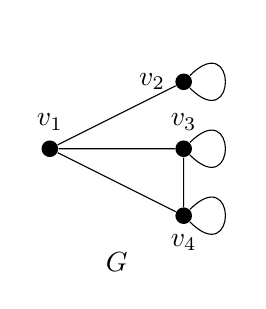
\begin{tikzpicture}[scale=0.85, vertex/.style={minimum width=6pt, circle, inner sep=0pt}]
			\node at (0,-1.7){$G$};
			\node[vertex,fill,label=above:$v_1$] (1) at (-1,0) {};
			\node[vertex,fill,label=left:$v_2$] (2) at (1,1) {};
			\node[vertex,fill,label=above:$v_3$] (3) at (1,0) {};
			\node[vertex,fill,label=below:$v_4$] (4) at (1,-1) {};
			\draw (2) to [out=45, in=315, loop, min distance=1cm](2);
			\draw (3) to [out=45, in=315, loop, min distance=1cm](3);
			\draw (4) to [out=45, in=315, loop, min distance=1cm](4);
			\draw (2)--(1)--(3)--(4)--(1);
		\end{tikzpicture}
	\end{minipage}
	\hspace{2pt}
	\begin{minipage}{0.4\textwidth}
		\centering
		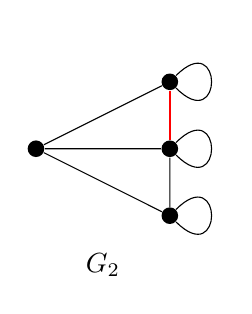
\begin{tikzpicture}[scale=0.85, vertex/.style={minimum width=6pt, circle, inner sep=0pt}]
			\node at (0,-1.74){$G_2$};
			\node[vertex,fill] (1) at (-1,0) {};
			\node[vertex,fill] (2) at (1,1) {};
			\node[vertex,fill] (3) at (1,0) {};
			\node[vertex,fill] (4) at (1,-1) {};
			\draw (2) to [out=45, in=315, loop, min distance=1cm](2);
			\draw (3) to [out=45, in=315, loop, min distance=1cm](3);
			\draw (4) to [out=45, in=315, loop, min distance=1cm](4);
			\draw (2)--(1)--(3)--(4)--(1);
			\draw[thick,red] (2)--(3);
		\end{tikzpicture}
	\end{minipage}
	\caption{Graphs: $G$ and $G_2$.}
	\label{fig:gandmc}
\end{figure}


\begin{figure}[htbp]
	\centering
	\begin{minipage}{0.45\textwidth}
		\centering
		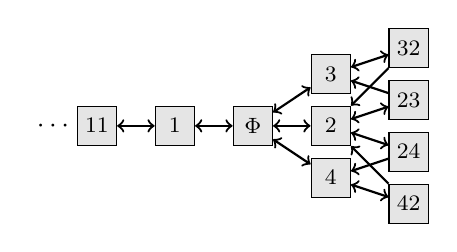
\begin{tikzpicture}[scale=0.66, state/.style={minimum width=5mm, minimum height=5mm, draw=black, fill=gray!20, inner sep=0pt, font=\footnotesize}]
			\node[state] (0) at (0,0) {$\Phi$};
			\node[state] (1) at (-1.5,0) {$1$};
			\node[state] (11) at (-3,0) {$11$};
			\node (111) at (-3.8,0) {$\cdots$};
			\node[state] (3) at (1.5,1) {$3$};
			\node[state] (2) at (1.5,0) {$2$};
			\node[state] (4) at (1.5,-1) {$4$};
			\node[state] (32) at (3,1.5) {$32$};
			\node[state] (23) at (3,0.5) {$23$};
			\node[state] (24) at (3,-0.5) {$24$};
			\node[state] (42) at (3,-1.5) {$42$};
			
			\draw[thick,<->](0)--(1);
			\draw[thick,<->](11)--(1);
			\draw[thick,<->](0)--(3);
			\draw[thick,<->](0)--(2);
			\draw[thick,<->](0)--(4);
			\draw[thick,<->](3)--(32);
			\draw[thick,<->](2)--(24);
			\draw[thick,<->](2)--(23);
			\draw[thick,<->](4)--(42);
			\draw[thick,->](32)--(2);
			\draw[thick,->](42)--(2);
			\draw[thick,->](23)--(3);
			\draw[thick,->](24)--(4);
		\end{tikzpicture}
	\end{minipage}
	\vspace{2pt}
	\begin{minipage}{0.45\textwidth}
		\centering
		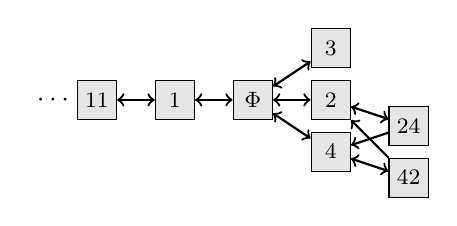
\begin{tikzpicture}[scale=0.66, state/.style={minimum width=5mm, minimum height=5mm, draw=black, fill=gray!20, inner sep=0pt, font=\footnotesize}]
			\node[state] (0) at (0,0) {$\Phi$};
			\node[state] (1) at (-1.5,0) {$1$};
			\node[state] (11) at (-3,0) {$11$};
			\node (111) at (-3.8,0) {$\cdots$};
			\node[state] (3) at (1.5,1) {$3$};
			\node[state] (2) at (1.5,0) {$2$};
			\node[state] (4) at (1.5,-1) {$4$};
			%\node[state] (32) at (3,1.5) {$32$};
			%\node[state] (23) at (3,0.5) {$23$};
			\node[state] (24) at (3,-0.5) {$24$};
			\node[state] (42) at (3,-1.5) {$42$};
			
			\draw[thick,<->](0)--(1);
			\draw[thick,<->](11)--(1);
			\draw[thick,<->](0)--(3);
			\draw[thick,<->](0)--(2);
			\draw[thick,<->](0)--(4);
			%\draw[thick,<->](3)--(32);
			\draw[thick,<->](2)--(24);
			%\draw[thick,<->](2)--(23);
			\draw[thick,<->](4)--(42);
			%\draw[thick,red,->](32)--(2);
			\draw[thick,->](42)--(2);
			%\draw[thick,red,->](23)--(3);
			\draw[thick,->](24)--(4);
		\end{tikzpicture}
	\end{minipage}
	\caption{Truncation of the Markov Chains for $G$ (left) and  $G_2$ (right).}
	\label{fig:mc}
\end{figure}



We consider $G=(\mathcal{V},\mathcal{E})$ in Fig.~\ref{fig:gandmc}, where $\mathcal{V}$ is partitioned into $\mathcal{V}_1=\{v_2, v_3, v_4\}$ and $\mathcal{V}_2=\{v_1\}$. The independent sets of $\check{G}$ are 
$
\{\{v_1\}, \{v_2\}, \{v_3\}, \{v_4\}, \{v_2,v_4\}, \\
\{v_2,v_3\}\}
$.
Graph $G_2$ is 
obtained by inserting the edge $\{v_2,v_3\}$ (see Fig.~\ref{fig:gandmc}). The associated Markov Chains, 
truncated to states with at most two letters, are depicted in Fig.~\ref{fig:mc}. 
The rates are 
$\lambda_1 = 0.432685$, 
$\lambda_2 = 0.005861$, $\lambda_3 = 0.141128$ and 
$\lambda_4 = 0.420326$. The BS set is a singleton (i.e. $\{v1\})$. 
We have a paradox as the expectation slightly increases from 
$2.944793$ to $2.947256$ when we add the edge. 



The former example does not address the case of adding a new edge $e$ connecting a node lacking a self-loop to a node with self-loop. To fill this gap, we study graph $H_2$ (see Fig.\ref{fig:graphs_example2}),  obtained from $H$ by inserting edge $\{v_1,v_5\}$. Similarly, graph $H_1$ is formed by connecting $v_2$ and $v_3$, while graph $H_3$ is obtained by adding a self-loop to {$v_5$}. We have found performance paradoxes in all cases.
For arrival rate vector 
$( 0.070716, 0.180906, 0.238414, 0.204521,  0.164007, 0.07243, 
0.069006)$
the bottleneck set is $\{v_7\}$. The expectation is $31.218542$ for graph $H$ 
and it increases to 
$ 31.539906$ for graph $H_1$.  
Similarly, if we start with arrival rate vector 
$( 0.08502,  0.06418,  0.076071,  0.096493,  0.336406, 0.326572, 0.015258)$
for $H$, we get an expectation for the total number equal to $13.0179$ and the expectation is equal to $13.058815$ for the same rates and graph $H_2$. Finally, 
the comparison between $H$ and $H_3$ for rate vector $(0.104627, 0.052725,  0.194586, 0.190934, 0.117413, 0.225466,\\ 0.114249)$ also shows a performance
paradox: the expectation was $33.838547$ for $H$ and it jumps to $35.972599$ for $H_3$. In both cases, the bottleneck independent  set is singleton $\{v_6 \}$. 

\begin{figure}[htbp]
	\centering
	\begin{minipage}{0.22\textwidth}
		\centering
		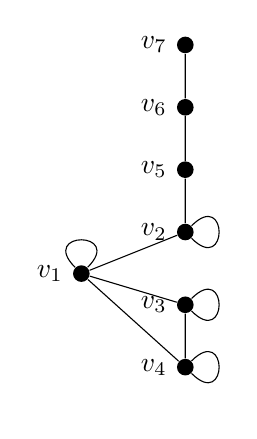
\begin{tikzpicture}[scale=0.66, vertex/.style={minimum width=6pt, circle, inner sep=0pt}]
			\node[vertex,fill, label=left:$v_1$](1) at (-1,0){};
			\node[vertex,fill, label=left:$v_2$](2) at (1,0.8){};
			\node[vertex,fill, label=left:$v_3$](3) at (1,-0.6){};
			\node[vertex,fill, label=left:$v_4$](4) at (1,-1.8){};
			\node[vertex,fill, label=left:$v_5$](5) at (1,2){};
			\node[vertex,fill, label=left:$v_6$](6) at (1,3.2){};
			\node[vertex,fill, label=left:$v_7$](7) at (1,4.4){};
			\draw (1) to [out=45, in=135, loop, min distance=1cm](1);
			\draw (2) to [out=45, in=315, loop, min distance=1cm](2);
			\draw (3) to [out=45, in=315, loop, min distance=1cm](3);
			\draw (4) to [out=45, in=315, loop, min distance=1cm](4);
			%\draw (5) to [out=45, in=315, loop, min distance=1cm](5);
			\draw(1)--(3)--(4)--(1)--(2)--(5)--(6)--(7);
		\end{tikzpicture}
	\end{minipage}
	\hspace{2pt}
	\begin{minipage}{0.22\textwidth}
		\centering
		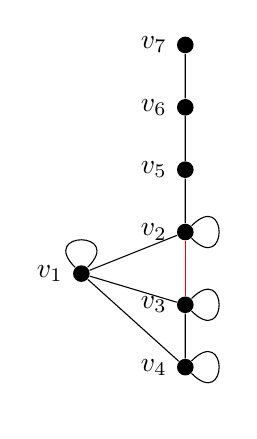
\begin{tikzpicture}[scale=0.66, vertex/.style={minimum width=6pt, circle, inner sep=0pt}]
			\node[vertex,fill, label=left:$v_1$](1) at (-1,0){};
			\node[vertex,fill, label=left:$v_2$](2) at (1,0.8){};
			\node[vertex,fill, label=left:$v_3$](3) at (1,-0.6){};
			\node[vertex,fill, label=left:$v_4$](4) at (1,-1.8){};
			\node[vertex,fill, label=left:$v_5$](5) at (1,2){};
			\node[vertex,fill, label=left:$v_6$](6) at (1,3.2){};
			\node[vertex,fill, label=left:$v_7$](7) at (1,4.4){};
			\draw (1) to [out=45, in=135, loop, min distance=1cm](1);
			\draw (2) to [out=45, in=315, loop, min distance=1cm](2);
			\draw (3) to [out=45, in=315, loop, min distance=1cm](3);
			\draw (4) to [out=45, in=315, loop, min distance=1cm](4);
			%\draw (5) to [out=45, in=315, loop, min distance=1cm](5);
			\draw(1)--(3)--(4)--(1)--(2)--(5)--(6)--(7);
			\draw[red] (2)--(3);
		\end{tikzpicture}
	\end{minipage}
	\hspace{2pt}
	\begin{minipage}{0.22\textwidth}
		\centering
		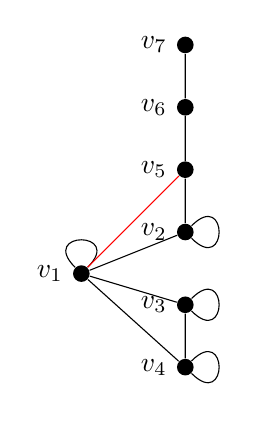
\begin{tikzpicture}[scale=0.66, vertex/.style={minimum width=6pt, circle, inner sep=0pt}]
			\node[vertex,fill, label=left:$v_1$](1) at (-1,0){};
			\node[vertex,fill, label=left:$v_2$](2) at (1,0.8){};
			\node[vertex,fill, label=left:$v_3$](3) at (1,-0.6){};
			\node[vertex,fill, label=left:$v_4$](4) at (1,-1.8){};
			\node[vertex,fill, label=left:$v_5$](5) at (1,2){};
			\node[vertex,fill, label=left:$v_6$](6) at (1,3.2){};
			\node[vertex,fill, label=left:$v_7$](7) at (1,4.4){};
			\draw (1) to [out=45, in=135, loop, min distance=1cm](1);
			\draw (2) to [out=45, in=315, loop, min distance=1cm](2);
			\draw (3) to [out=45, in=315, loop, min distance=1cm](3);
			\draw (4) to [out=45, in=315, loop, min distance=1cm](4);
			%\draw (5) to [out=45, in=315, loop, min distance=1cm](5);
			\draw(1)--(3)--(4)--(1)--(2)--(5)--(6)--(7);
			\draw[red](1)--(5);
		\end{tikzpicture}
	\end{minipage}
	\hspace{2pt}
	\begin{minipage}{0.22\textwidth}
		\centering
		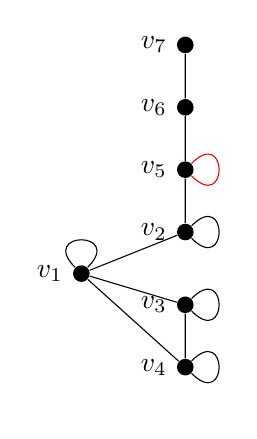
\begin{tikzpicture}[scale=0.66, vertex/.style={minimum width=6pt, circle, inner sep=0pt}]
			\node[vertex,fill, label=left:$v_1$](1) at (-1,0){};
			\node[vertex,fill, label=left:$v_2$](2) at (1,0.8){};
			\node[vertex,fill, label=left:$v_3$](3) at (1,-0.6){};
			\node[vertex,fill, label=left:$v_4$](4) at (1,-1.8){};
			\node[vertex,fill, label=left:$v_5$](5) at (1,2){};
			\node[vertex,fill, label=left:$v_6$](6) at (1,3.2){};
			\node[vertex,fill, label=left:$v_7$](7) at (1,4.4){};
			\draw (1) to [out=45, in=135, loop, min distance=1cm](1);
			\draw (2) to [out=45, in=315, loop, min distance=1cm](2);
			\draw (3) to [out=45, in=315, loop, min distance=1cm](3);
			\draw (4) to [out=45, in=315, loop, min distance=1cm](4);
			\draw[red] (5) to [out=45, in=315, loop, min distance=1cm](5);
			\draw(1)--(3)--(4)--(1)--(2)--(5)--(6)--(7);
		\end{tikzpicture}
	\end{minipage}
	\caption{graphs: $H$, $H_1$, $H_2$ and $H_3$. }
	\label{fig:graphs_example2}
\end{figure}

\paragraph{Open question.}
When all nodes are looped ($V_1=V$), does \eqref{eq:exp-multi} admit further simplification or monotonicity properties under edge additions?


\section{Performance paradox in matching models with abandonment}\label{sec:abandonment}
We extend the model to allow abandonments. Items of class $i\in V$ arrive as independent Poisson processes with rates $\mu_i$ (normalized so that $\mu(V)=\sum_{i\in V}\mu_i=1$). Under \textsc{FCFM}, when an arrival finds a compatible item stored, the oldest such item is removed together with the arrival; otherwise the item is stored. In addition, each stored item of class $i$ abandons independently at rate $\delta_i>0$. For the closed–form analyses below we work with the same abandonment $\delta_i\equiv\delta>0$.
For general graphs, a closed product form is not available; however, for the complete graph $K_n$ and the graph $K_n-\{1,2\}$, the steady state can be characterised explicitly, and the latter reduces to $K_{n-1}$ by strong lumpability.

\begin{contribution}{ $K_n$ (ergodicity and steady state)}
	On the complete graph $K_n$ with abandonment $\delta>0$, the \textsc{FCFM} CTMC decomposes into $n$ birth–death (BD) components that are connected only through the empty state. Writing $\beta_i:=\sum_{j\neq i}\mu_j=1-\mu_i$, the stationary probabilities of the BD chain that counts class–$i$ items are
	\begin{equation}\label{eq:pi-im-Kn}
		\pi_{i,m}\;=\;\pi_{\emptyset}^{(\delta)}\prod_{k=1}^{m}\frac{\mu_i}{\beta_i+k\delta},\qquad m\ge 1,\ \ i=1,\dots,n,
	\end{equation}
	with the empty–state normalizer
	\begin{equation}\label{eq:pi0-Kn}
		\bigl(\pi_{\emptyset}^{(\delta)}\bigr)^{-1}\;=\;1+\sum_{i=1}^{n}\ \sum_{m=1}^{\infty}\ \prod_{k=1}^{m}\frac{\mu_i}{\beta_i+k\delta}.
	\end{equation}
	Consequently,
	\begin{equation}\label{eq:EV-Kn-delta}
		\mathbb{E}[K_n,\mu,\delta]\;=\;\sum_{i=1}^{n}\ \sum_{m=1}^{\infty}\ m\,\pi_{\emptyset}^{(\delta)}\prod_{k=1}^{m}\frac{\mu_i}{\beta_i+k\delta}.
	\end{equation}
\end{contribution}

\begin{proof}[Proof]
	On $K_n$ any admissible word contains a single letter type, hence from a nonempty state $(i,m)$ the only moves are $(i,m)\to(i,m+1)$ at rate $\mu_i$ (arrival of $i$), $(i,m)\to(i,m-1)$ at rate $\beta_i$ (arrival of any $j\neq i$ that matches the oldest $i$), and $(i,m)\to(i,m-1)$ at rate $m\delta$ (one of the $m$ items abandons). Local balance on the BD line yields \eqref{eq:pi-im-Kn}. Summing masses including the empty state gives \eqref{eq:pi0-Kn}; linearity yields \eqref{eq:EV-Kn-delta}. 
	\emph{Ergodicity:} since $\beta_i>0$ and $\delta>0$, $\sum_{m\ge1}\prod_{k=1}^{m}\mu_i/(\beta_i+k\delta)\le \sum_{m\ge1}(\mu_i/\delta)^m/m!<\infty$, so the series in \eqref{eq:pi0-Kn} converges and the chain is positive recurrent.
\end{proof}

\begin{contribution}{$K_n-\{1,2\}$ (strong lumpability to $K_{n-1}$)}
	Let $G=K_n-\{1,2\}$ and assume $\delta>0$ and $\beta_1=\beta_2=\sum_{j\ge3}\mu_j$. Consider the partition $\mathcal{E}=\{B_{\emptyset}\}\cup\{B_{i,m}: i\ge3,\ m\ge1\}\cup\{B_{12,k}:k\ge1\}$ where $B_{\emptyset}=\{\emptyset\}$, $B_{i,m}$ is the singleton $\{i^m\}$ for $i\ge3$, and $B_{12,k}$ collects all words of length $k$ with letters only from $\{1,2\}$ in any order. Then the CTMC is \emph{strongly lumpable} with respect to $\mathcal{E}$ in the sense of Ball–Yeo, and the lumped chain is isomorphic to the $K_{n-1}$ model obtained by merging $1$ and $2$ into a single vertex $a$ with arrival rate
	\[
	\mu'_a=\mu_1+\mu_2,\qquad \mu'_i=\mu_i\ (i\ge3),\qquad \delta'_a=\delta'_i=\delta.
	\]
	In particular,
	\begin{equation}\label{eq:EV-Kn12-equals-Kn-1}
		\mathbb{E}[K_n-\{1,2\},\mu,\delta]\;=\;\mathbb{E}[K_{n-1},\mu',\delta].
	\end{equation}
\end{contribution}

\begin{proof}[Proof (Ball–Yeo strong lumpability and jumpability\cite{BaYe93})]
	\emph{(i) Regularity/irreducibility/positive recurrence)} Let $Z$ be the embedded chain and $V(w)$ the word length. From any nonempty state, with positive probability the next jump is a departure (match or abandonment), so $\mathbb{E}[\Delta V\mid V=k]\le (\sum_i\mu_i-k\delta)/(\sum_i\mu_i+k\delta)$, which is $<-1/2$ for all sufficiently large $k$. By Foster–Lyapunov, $Z$ is positive recurrent; hence the CTMC is regular and positive recurrent (standard results on embedded chains).
	
	\emph{(ii) Strong lumpability)} For any $w\in B_{12,k}$, the total rates from $w$ to the blocks of the partition are:
	\[
	q\bigl(w,B_{12,k+1}\bigr)=\mu_1+\mu_2,\quad
	q\bigl(w,B_{12,k-1}\bigr)=k\delta,\quad
	q\bigl(w,B_{\emptyset}\bigr)=\mathbf{1}_{\{k=1\}}\beta_1,\quad
	q\bigl(w,B_{i,1}\bigr)=\mu_i\ \ (i\ge3).
	\]
	These depend only on $k$ (not on the internal order of 1s and 2s), and for $i\ge3$ the singletons $B_{i,m}$ and $B_{\emptyset}$ are trivial blocks. Therefore the Ball–Yeo column–sum condition $Q_{i,j}\mathbf{1}=\lambda_{i,j}\mathbf{1}$ holds for all block pairs, yielding strong lumpability. The lumped chain has the same transition structure as $K_{n-1}$ where $\{1,2\}$ is merged into $a$, hence \eqref{eq:EV-Kn12-equals-Kn-1}. The same blockwise constancy shows the chain is \emph{jumpable} (block–to–block rates are constant across micro–states).
\end{proof}
Having established closed-form series for $K_n$
and the lumpability reduction for 
$K_n-\{1,2\}$, we now give a certified truncation scheme for evaluating 
$\pi_{\emptyset}^{(\delta)}$
and 
$\mathbb{E}[Q_i]$
to a prescribed accuracy.
\begin{contribution}{Truncated–series evaluation with error control}
	Define, for $i=1,\dots,n$,
	\[
	S_i\ :=\ \sum_{m=1}^{\infty}\ \prod_{k=1}^{m}\frac{\mu_i}{\beta_i+k\delta},\qquad
	S_i(N)\ :=\ \sum_{m=1}^{N}\ \prod_{k=1}^{m}\frac{\mu_i}{\beta_i+k\delta},\qquad
	R_i(N):=S_i-S_i(N).
	\]
	\textbf{Case A:} if $\delta>\mu_i$, then $R_i(N)\le \sum_{m\ge N+1}(\mu_i/\delta)^m/m!\le 1/(N!)$.  
	\textbf{Case B:} if $\delta\le \mu_i$, let $P=\min\{p\in\mathbb{N}: \mu_i<p\delta\}$. Using
	\[
	\prod_{k=1}^{m}\frac{\mu_i}{\beta_i+k\delta}\ \le\ 
	\Bigl(\frac{\mu_i}{\beta_i+\delta}\Bigr)^{\!P}
	\Bigl(\frac{\mu_i}{P\delta}\Bigr)^{\!m-P},
	\]
	we obtain $R_i(N)\le \bigl(\frac{\mu_i}{\beta_i+\delta}\bigr)^{P}\bigl(\frac{\mu_i}{P\delta}\bigr)^{N+1-P}\big/\bigl(1-\frac{\mu_i}{P\delta}\bigr)$.  
	Given a target tolerance $\varepsilon>0$, choose $N_i$ so that $R_i(N_i)\le \varepsilon/n$ by the appropriate case; set $N=\max_i N_i$. Then
	\begin{equation}\label{eq:pi0-bounds}
		\pi_{\emptyset}^{(\delta)}\ \le\ \Bigl(1+\sum_{i=1}^{n}S_i(N)\Bigr)^{-1}\ =:\ \overline{\pi}_{\emptyset}^{(\delta)},\qquad
		0\ \le\ \overline{\pi}_{\emptyset}^{(\delta)}-\pi_{\emptyset}^{(\delta)}\ <\ \varepsilon,
	\end{equation}
	and
	\begin{equation}\label{eq:EV-bounds}
		\underline{\mathbb{E}}[K_n,\mu,\delta]\ :=\ \sum_{i=1}^{n}\sum_{m=1}^{N+1}m\,\overline{\pi}_{\emptyset}^{(\delta)}\prod_{k=1}^{m}\frac{\mu_i}{\beta_i+k\delta}
		\ \le\ \mathbb{E}[K_n,\mu,\delta]\ \le\
		\underline{\mathbb{E}}[K_n,\mu,\delta]\ +\ \frac{\varepsilon}{\delta}\sum_{i=1}^{n}\mu_i,
	\end{equation}
	where the tail term uses $\pi_{\emptyset}^{(\delta)}\le1$ and $m\,\mu_i/(\beta_i+m\delta)\le \mu_i/\delta$.  
	For $K_n-\{1,2\}$, combine \eqref{eq:EV-Kn12-equals-Kn-1} with \eqref{eq:pi0-bounds}–\eqref{eq:EV-bounds} for the lumped instance $(K_{n-1},\mu',\delta)$. 
\end{contribution}

\paragraph{Remarks.}
Certified implementations of the truncation scheme and Monte Carlo search for paradox instances under abandonment are provided in our repository \cite{li2025a}.


\section{Performance paradox in matching models with cost}\label{sec:cost}
Given class-dependent holding-cost rates $c=(c_i)_{i\in V}$ with $c_i>0$, we evaluate performance under \textsc{FCFM} via the stationary expected total holding cost
\begin{equation}\label{eq:def-cost}
	E[G,\mu,c]:=\sum_{i\in V} c_i\mathbb{E}[Q_i],
\end{equation}
where $Q_i$ is the total number of item $i$ and expectations are taken with respect to the product-form stationary distribution when the chain is positive recurrent.

%\subsection{Complete graph $K_n$}\label{subsec:Kn}
On $K_n$ any two distinct classes are compatible. By \eqref{eq:product-form}–\eqref{eq:pi0-general}, only single-letter words are admissible; hence the total number of $i$ in the buffer are geometric.

\begin{contribution}[Closed form on $K_n$]\label{prop:Kn}
	Assume \textsc{NCOND} (equivalently $\mu_i<\mu(\Gamma_i)=\sum_{j\neq i}\mu_j$ for all $i$).
	Then
	\begin{equation}\label{eq:KnCost}
		E[K_n,\mu,c]=\pi_{\emptyset}\sum_{i=1}^n\frac{c_i\,\mu(\Gamma_i)\,\mu_i}{\bigl(\mu(\Gamma_i)-\mu_i\bigr)^2},
		\qquad
		\pi_{\emptyset}
		=\Bigl(1+\sum_{i=1}^n \frac{\mu_i}{\mu(\Gamma_i)-\mu_i}\Bigr)^{-1}.
	\end{equation}
\end{contribution}

\begin{proof}
	By the product-form result for the general matching model (see Theorem~\ref{thm:pf-simple}),
	the normalizing constant on a general graph is a finite sum over independent sets.
	On $K_n$, independent sets are exactly the singletons $\{i\}$, $i=1,2,\dots,n$; thus the normalization reduces to \eqref{eq:KnCost}.
	
	Fix a class $i$. As argued above, any admissible state containing only class-$i$ items is
	a word of length $m\ge 0$, with stationary weight proportional to $\bigl(\mu_i/\mu(\Gamma_i)\bigr)^m$.
	Hence the class-$i$ queue-length distribution is geometric, and its contribution to the
	expected holding cost equals
	\[
	\pi_\emptyset \sum_{m=0}^{\infty} \Bigl(\frac{\mu_i}{\mu(\Gamma_i)}\Bigr)^{m} \, m\, c_i
	=\pi_\emptyset \, c_i \,\frac{\mu_i}{\mu(\Gamma_i)}
	\frac{1}{\Bigl(1-\frac{\mu_i}{\mu(\Gamma_i)}\Bigr)^2},
	\]
	where we used Geometric first-moment identity. Summing over $i=1,\dots,n$ gives \eqref{eq:KnCost}.
\end{proof}

%\subsection{Edge-deleted graph $K_n-\{1,2\}$}\label{subsec:Kn12}
On $K_n-\{1,2\}$, here $\Gamma_1=\Gamma_2=\{3,\dots,n\}$ so that $\mu(\Gamma_1)=\mu(\Gamma_2)=\mu(\Gamma(\{1,2\}))$; classes $1$ and $2$ cannot match each other and may coexist.

\begin{contribution}[Closed form on $K_n-\{1,2\}$]\label{prop:Kn12}
	Assume \textsc{NCOND}. Then
	\begin{equation}\label{eq:KnMinusCost}
		E[K_n-\{1,2\},\mu,c]
		\;=\;
		\pi_{\emptyset}\Biggl(
		\sum_{i=3}^n \frac{c_i\,\mu(\Gamma_i)\,\mu_i}{\bigl(\mu(\Gamma_i)-\mu_i\bigr)^2}+\frac{\mu(\Gamma_1)\,\bigl(c_1\mu_1+c_2\mu_2\bigr)}
		{\bigl(\mu(\Gamma_1)-\mu_1-\mu_2\bigr)^2}
		\Biggr),
	\end{equation}
	with
	\begin{equation}\label{eq:pi0KnMinus}
		\pi_{\emptyset}
		=\Biggl(1+\sum_{i=1}^n \frac{\mu_i}{\mu(\Gamma_i)-\mu_i}
		+\frac{\mu_1\mu_2}{(\mu(\Gamma_1)-\mu_1)(\mu(\Gamma_1)-\mu_1-\mu_2)}
		+\frac{\mu_1\mu_2}{(\mu(\Gamma_1)-\mu_2)(\mu(\Gamma_1)-\mu_1-\mu_2)}\Biggr)^{-1}.
	\end{equation}
\end{contribution}

\begin{proof}
	As in the complete-graph case, we begin from the general product-form expression 
	(see Theorem~\ref{thm:pf-simple}). 
	On $K_n-\{1,2\}$ the independent sets consist of:
	(i) each singleton $\{i\}$, $i=1,\dots,n$; and (ii) the pair $\{1,2\}$, since nodes~1 and~2 are no longer adjacent. 
	Since $\Gamma_1=\Gamma_2=\Gamma(\{1,2\})$, then this additional independent set $\{1,2\}$ introduces the cross-term in~\eqref{eq:pi0KnMinus}.
	
	For nodes $i\geq 3$, the computation of the expected cost contribution is identical to the 
	complete-graph case: the total number of each class-$i$ in the buffer is geometric with mean given by Geometric first-moment identity, yielding the first summation in~\eqref{eq:KnMinusCost}.
	
	For nodes 1 and 2, however, class-$i$ may coexist because they cannot match each other. 
	Thus admissible states include words of the form $1^{m_1}2^{m_2}$ for $m_1,m_2\ge 0$. 
	Their stationary weight is proportional to
	$$
	\binom{m_1+m_2}{m_1}
	\left(\frac{\mu_1}{\mu(\Gamma_1)}\right)^{m_1}
	\left(\frac{\mu_2}{\mu(\Gamma_2)}\right)^{m_2},
	$$
	reflecting the order-preserving FCFM discipline. Multiplying by the cost 
	$m_1 c_1 + m_2 c_2$ and summing over all $m_1,m_2\ge 0$ yields exactly the bivariate 
	series in Bivariate binomial-convolution identities with parameters 
	$r_1=\mu_1/\mu(\Gamma_1)$, $r_2=\mu_2/\mu(\Gamma_2)$. 
Bivariate binomial-convolution identities then gives
	\begin{equation}
		\sum_{m_1,m_2\geq0}
		\binom{m_1+m_2}{m_1} 
		\left(\frac{\mu_1}{\mu(\Gamma_1)}\right)^{m_1}
		\left(\frac{\mu_2}{\mu(\Gamma_2)}\right)^{m_2}
		(m_1 c_1+m_2 c_2)
		=\frac{\frac{c_1\mu_1}{\mu(\Gamma_1)}+\frac{c_2\mu_2}{\mu(\Gamma_2)}}{(1-\frac{\mu_1}{\mu(\Gamma_1)}-\frac{\mu_2}{\mu(\Gamma_2)})^2}.
	\end{equation}
	Multiplying numerator and denominator by $\mu(\Gamma_1)\mu(\Gamma_2)$, 
	and using that $\mu(\Gamma_1)=\mu(\Gamma_2)$ by symmetry of the complete graph minus 
	one edge, we obtain the second term of \eqref{eq:KnMinusCost}.
\end{proof}

Formulas \eqref{eq:KnCost}–\eqref{eq:KnMinusCost} enable direct cost comparisons on $K_n$ vs.\ $K_n-\{1,2\}$ under the same $(\mu,c)$ and $\mu(V)=1$. In Section~\ref{subsec:paracost} we report parameter regions where $E[K_5,\mu,c]>E[K_5-\{1,2\},\mu,c]$ (or the reverse).

\subsection{Paradox with cost for $K_5$ and $K_5-\{1,2\}$}\label{subsec:paracost}
\begin{figure} [htbp]
	\begin{center} 
		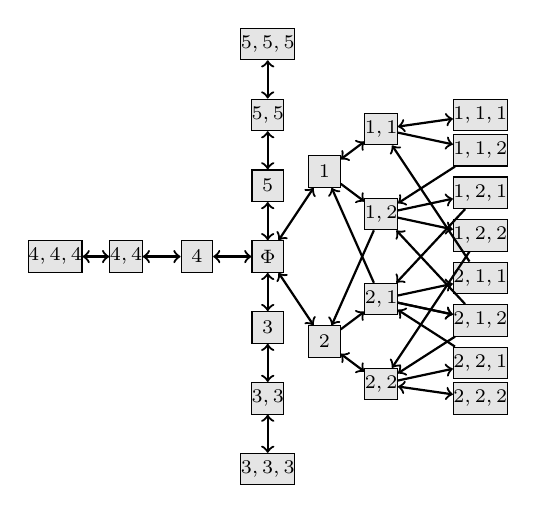
\begin{tikzpicture}[scale=0.9, state/.style={minimum width=4mm, minimum height=4mm, draw=black, fill=gray!20, inner sep=0pt, font=\scriptsize}]
			
			\node[state] (0) at (0,0)  {$\Phi$};
			
			\node[state] (5) at (0,1)  {$5$};
			\node[state] (55) at (0,2)  {$5,5$};
			\node[state] (555) at (0,3)  {$5,5,5$};
			
			\node[state] (3) at (0,-1)  {$3$};
			\node[state] (33) at (0,-2)  {$3,3$};
			\node[state] (333) at (0,-3)  {$3,3,3$};
			
			\node[state] (4) at (-1,0)  {$4$};
			\node[state] (44) at (-2,0)  {$4,4$};
			\node[state] (444) at (-3,0)  {$4,4,4$};
			
			\draw[<->, thick] (444)--(44);
			\draw[<->, thick] (333)--(33);
			\draw[<->, thick] (555)--(55);
			
			\foreach \x /\y in {44/4, 4/0, 55/5, 5/0, 0/3, 3/33}
			{\draw[<->, thick] (\x)--(\y);}
			
			\node[state] (1) at (0.8,1.2)  {$1$};
			\node[state] (2) at (0.8,-1.2)  {$2$};
			
			\node[state] (11) at (1.6,1.8)  {$1,1$};
			\node[state] (12) at (1.6,0.6)  {$1,2$};
			\node[state] (21) at (1.6,-0.6)  {$2,1$};
			\node[state] (22) at (1.6,-1.8)  {$2,2$};
			
			\draw[<->, thick] (0)--(1);
			\draw[<->, thick] (0)--(2);
			
			\draw[<->, thick] (1)--(11);
			\draw[->, thick] (1)--(12);
			\draw[->, thick] (21)--(1);
			\draw[->, thick] (2)--(21);
			\draw[<->, thick] (2)--(22);
			\draw[->, thick] (12)--(2);
			
			\node[state] (111) at (3,2.0)  {$1,1,1$};
			\node[state] (112) at (3,1.5)  {$1,1,2$};
			\node[state] (121) at (3,0.9)  {$1,2,1$};
			\node[state] (122) at (3,0.3)  {$1,2,2$};
			\node[state] (211) at (3,-0.3)  {$2,1,1$};
			\node[state] (212) at (3,-0.9)  {$2,1,2$};
			\node[state] (221) at (3,-1.5)  {$2,2,1$};
			\node[state] (222) at (3,-2)  {$2,2,2$};
			
			\foreach \a/\b in {11/111, 22/222} {
				\draw[<->, thick] (\a)--(\b);
			}
			
			\draw[->, thick] (11)--(112);
			\draw[->, thick] (22)--(221);
			\draw[->, thick] (21)--(212);
			
			\foreach \a/\b in {11/211, 12/112, 21/121, 21/221, 22/122, 22/212, 12/212} {
				\draw[<-, thick] (\a)--(\b);
			}
			
			\foreach \a/\b in {12/121, 12/122, 21/211,21/212} {
				\draw[->, thick] (\a)--(\b);
			}
		\end{tikzpicture}
	\end{center}
	\caption{CTMC for $K_5-\{1,2\}$, restricted to states with less than $4$ items. \label{secondmodel}}
\end{figure}
With the arrival rates: $\mu_1=0.2123089053707668$, $\mu_2=0.2742714546697317$,
$\mu_3=0.006999635670957356$,
$\mu_4=0.009689658354828117$,
$\mu_5=0.4967303459337161$,
we consider the cost rates:
$c_1=2.7238918756873907$,
$c_2=2.4122427717406985$,
$c_3=0.7902759709551836$,
$c_4=1.6367962372371867$,
$c_5=2.941675109364959$. Our
algorithms provide $\mathbb{E}[K_5]=220.65202293442172$ and $\mathbb{E}[K_5-\{1,2\}]=190.10942991220702$.

With the arrival rates: $\mu_1=0.3636329852744427$, $\mu_2=0.12673427390852054$,
$\mu_3=0.010843072513621425$,
$\mu_4=0.00588355294263528$,
$\mu_5=0.4967303459337161$,
we consider the cost rates:
$c_1=0.7586371655061703$,
$c_2=0.5922847832917051$,
$c_3=1.2921580773128705$,
$c_4=1.5334451333796428$,
$c_5=2.7928617067309602$. Our
algorithms provide $\mathbb{E}[K_5]=93.13740159182518$ and $\mathbb{E}[K_5-\{1,2\}]=64.52734567817744$.

With the arrival rates: $\mu_1=0.3318483989009918$, $\mu_2=0.15555361051577288$,
$\mu_3=0.008889036408139615$,
$\mu_4=0.010680845648430016$,
$\mu_5=0.4930281085266657$,
we consider the cost rates:
$c_1=0.540035985717008$,
$c_2=0.7140147194846248$,
$c_3=2.4159213267991975$,
$c_4=0.9251339822272417$,
$c_5=2.019825022348815$. Our
algorithms provide $\mathbb{E}[K_5]=69.11018350819715$ and $\mathbb{E}[K_5-\{1,2\}]=50.80578875204731$.

With the arrival rates: $\mu_1=0.27213894636867086$, $\mu_2=0.2103851356861736$,
$\mu_3=0.021582541556846437$,
$\mu_4=0.00206614868091172$,
$\mu_5=0.4938272277073974$,
we consider the cost rates:
$c_1=2.0706759633272456$,
$c_2=1.0160689586750364$,
$c_3=2.32274822225199$,
$c_4=1.2423689869742887$,
$c_5=2.4547513725489267$. Our
algorithms provide $\mathbb{E}[K_5]=95.94786753522975$ and $\mathbb{E}[K_5-\{1,2\}]=79.43003650548351$.



\section{Conclusions and Future Work}\label{sec:conclusions}

This report assembles three complementary results on performance paradoxes for stochastic matching under \textsc{FCFM}. (i) At the structural level, we give an explicit expected-value representation on multigraphs, together with its specialization to simple graphs, and use it to show that paradoxes arise beyond isolated examples—across a range of graph families that satisfy \textsc{NCOND}. (ii) At the objective level, we obtain closed-form evaluations on the benchmark pair $K_n$ and $K_n-\{1,2\}$ for $\mathbb{E}[G,\mu,c]$, including a refined empty-state normalization on $K_n-\{1,2\}$; these formulas enable exact side-by-side comparisons under a common $(\mu,c)$ and reveal sizable cost-weighted paradox regions. (iii) At the modeling level, for systems with abandonment we develop a phase-error approximation and, via strong lumpability, reduce $K_n-\{1,2\}$ to $K_{n-1}$ by aggregating $\{1,2\}$; this yields tractable evaluators for $\mathbb{E}[G,\mu,\delta]$ on the same benchmarks. Two themes recur throughout: independent-set bottlenecks—made visible by the denominators in the product-form expansions—and the value of evaluable expressions that turn structural product forms into computable performance measures.

Looking ahead, several threads are natural. First, \emph{applications}: (a) cross-trained service systems and skill-based routing, where adding a few cross-compatibilities to a predominantly bipartite core (creating small odd-cycle augmentations) is common practice; our resultes can inform whether a proposed compatibility edge is beneficial under given arrival mix; (b) substitution networks in assemble-to-order and inventory pooling, where partial substitutability induces compatibility graphs and the cost criterion $\mathbb{E}[G,\mu,c]$ is operationally meaningful; (c) redundancy-style computing and content delivery, which admit multigraph interpretations with self-loops and can be probed with the multigraph representation used here. Second, \emph{graph classes}: extend exact (or near-exact) evaluations beyond the two benchmarks to families that preserve tractable structure—e.g., $K_n$ minus a matching, $K_n$ minus a star, odd-cycle augmentations of bipartite cores, chordal and split graphs, and selected circulant or random graph models—seeking closed forms or controlled approximations. Third, \emph{design and policy}: formulate edge-addition/removal problems under $\mathbb{E}[G,\mu,c]$ as optimization tasks; examine sensitivity to tie-breaking and simple priority rules within \textsc{FCFM}; and refine the phase-error approximation by deriving error diagnostics or bounds and testing alternative patience embeddings. The computational artifacts for the present study (unweighted, cost-weighted, and abandonment settings) are released for reuse and extension; see \cite{li2025,li2025a,li2025b}.


\subsection*{Research plan for the next year}
% --- Aims (concise paragraphs) ---

\paragraph{Aim 1 (Policies on fully looped graphs).}
Identify matching policies under which paradoxes occur on multigraphs where every node has a self-loop ($V_1=V$). 

\paragraph{Aim 2 (Abandonment on general graphs).}
Extend the abandonment analysis from $K_n$ and $K_n-\{1,2\}$ to broader non-bipartite graph families. 

\paragraph{Aim 3 (Costs on general graphs).}
Move past the closed forms on $K_n$ and $K_n-\{1,2\}$ by developing computable expressions or bounds for $\mathbb{E}[G,\mu,c]$ on wider classes. Use the independent-set expansion to derive series representations; when exact summation is intractable, provide upper/lower bounds sufficient to detect cost-weighted paradoxes.

\paragraph{Aim 4 (Industrial applications).}
Translate the results into design guidance for cross-trained service systems and call centers (compatibility planning), assemble-to-order and substitution networks (component pooling), and redundancy-driven computing/content delivery (replica placement). Frame “which compatibilities to add/remove” under operational constraints using the evaluators developed here; release reproducible templates and code for practitioners.



\section{Academic Activities and Participation}\label{sec:activities}

This section summarizes my academic activities during the reporting period, including publications, research talks, conference participation, and editorial/reviewing service. The work disseminated in these venues consolidates three research threads under \textsc{FCFM}:

\begin{itemize}\itemsep0.25em
\item \emph{Performance paradoxes in matching systems are not that rare}. NETGCOOP 2025, Accepted.
\item \emph{Performance paradox in matching models with abandonment}. EAI VALUETOOLS 2025, Under review.
\item \emph{Performance paradox in matching models with cost}.
\end{itemize}
All code artifacts and configuration files are publicly released \cite{li2025,li2025a,li2025b}.

\paragraph{Talks and Posters.}
\begin{itemize}
\item Performance paradoxes in matching systems are not that rare, LINCS Annual Workshop, Palaiseau, France
\end{itemize}

\paragraph{Conference participation.}
\begin{itemize}\itemsep0.05em
\item Inhomogeneous random systems, Jan. 2025, Paris, France
\item AI Agent Reasoning and Decision-Making Workshop, Feb. 2025, Beijing(online), China
\item Annual workshop: Causal Modelling and Inference, Aug. 2025, Paris, France
\end{itemize}

\paragraph{Editorial and reviewing service.}
\begin{itemize}\itemsep0.25em
\item \textbf{Editorial board}. Member, \emph{Journal of Advances in Engineering and Technology}, since 2025.
\item \textbf{Reviewer (journals)}. \emph{Asian Journal of Mathematics and Computer Research}, \emph{Mathematics and Computer Science}, \emph{Journal of Advances in Mathematics and Computer Science}
\item \textbf{Reviewer (conferences)}. \emph{ICECET2025}, \emph{GPS2025}, \emph{ICIC2025}, \emph{ACDSA2025}.
\end{itemize}

\paragraph{Additional publications (outside dissertation scope).}
The following papers completed during the reporting period but not directly related to the dissertation topic were finalized and submitted in collaboration with external coauthors:
\begin{itemize}\itemsep0.25em
\item  A graph discretization of vector Laplacian. \textit{DAM}.
\item Extremal Spectral Radius of Trees with Fixed Eccentric Sequence. \textit{LAMA}, Under review. 
\item  Matrix-Tree Theorems for Complex Unit Gain Networks. \textit{JAMC}, Under review.
%\item ORKM: An R Package for Online Multi-View Data Clustering. \textit{NEUCOM}, Under review.
\end{itemize}

\bibliographystyle{abbrv}
\bibliography{references}

\end{document}

